%%
%% Copyright 2022 OXFORD UNIVERSITY PRESS
%%
%% This file is part of the 'oup-authoring-template Bundle'.
%% ---------------------------------------------
%%
%% It may be distributed under the conditions of the LaTeX Project Public
%% License, either version 1.2 of this license or (at your option) any
%% later version.  The latest version of this license is in
%%    http://www.latex-project.org/lppl.txt
%% and version 1.2 or later is part of all distributions of LaTeX
%% version 1999/12/01 or later.
%%
%% The list of all files belonging to the 'oup-authoring-template Bundle' is
%% given in the file `manifest.txt'.
%%
%% Template article for OXFORD UNIVERSITY PRESS's document class `oup-authoring-template'
%% with bibliographic references
%%

\documentclass[unnumsec,webpdf,modern,large,namedate]{oup-authoring-template}

\usepackage{float}
\usepackage{multicol}

\graphicspath{{figures/}}

\theoremstyle{thmstyleone}%
\newtheorem{theorem}{Theorem}%  meant for continuous numbers
%%\newtheorem{theorem}{Theorem}[section]% meant for sectionwise numbers
%% optional argument [theorem] produces theorem numbering sequence instead of independent numbers for Proposition
\newtheorem{proposition}[theorem]{Proposition}%
%%\newtheorem{proposition}{Proposition}% to get separate numbers for theorem and proposition etc.
\theoremstyle{thmstyletwo}%
\newtheorem{example}{Example}%
\newtheorem{remark}{Remark}%
\theoremstyle{thmstylethree}%
\newtheorem{definition}{Definition}

\begin{document}

%\subtitle{Subject Section}

\title[Supplementary Information]{Supplementary Information}

\author[1]{Justin Lin}
\author[2]{Julia Fukuyama}

\authormark{Lin and Fukuyama}

\begin{figure*}[t]
\centering
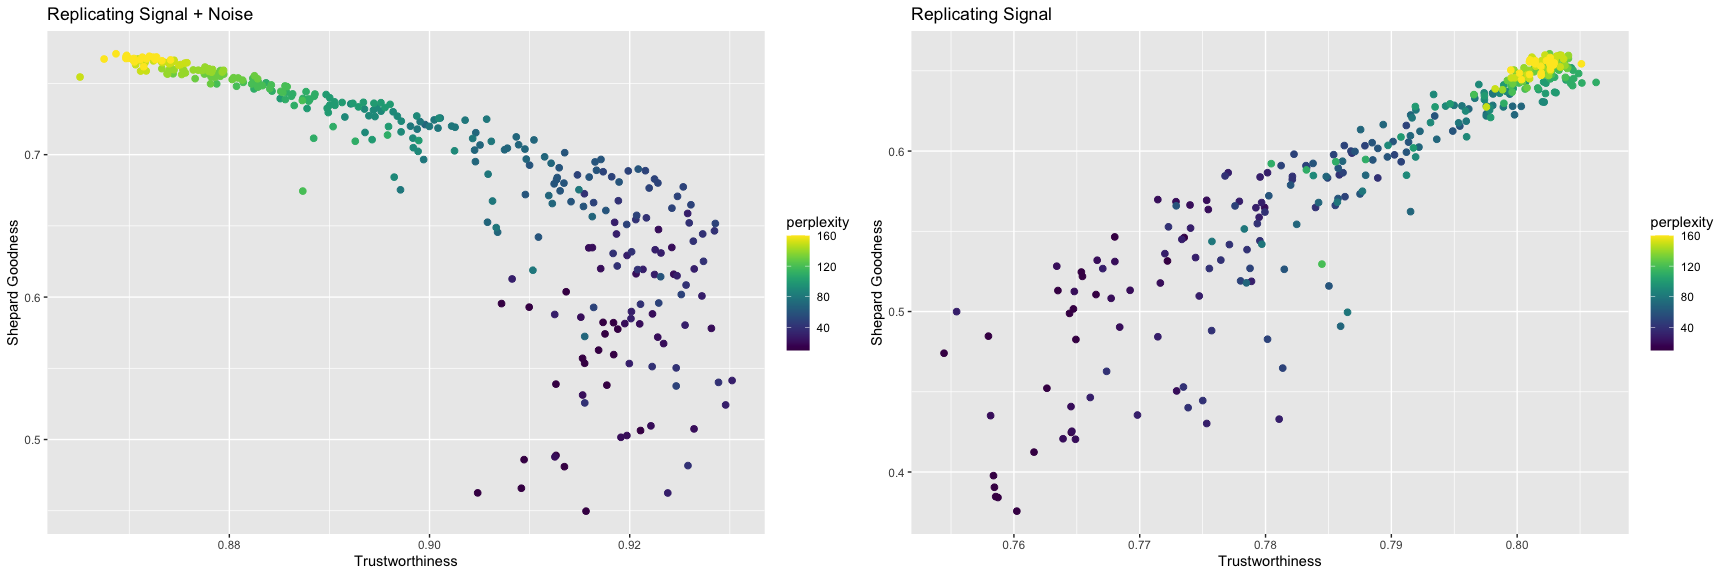
\includegraphics[scale=0.28]{trefoil plot}
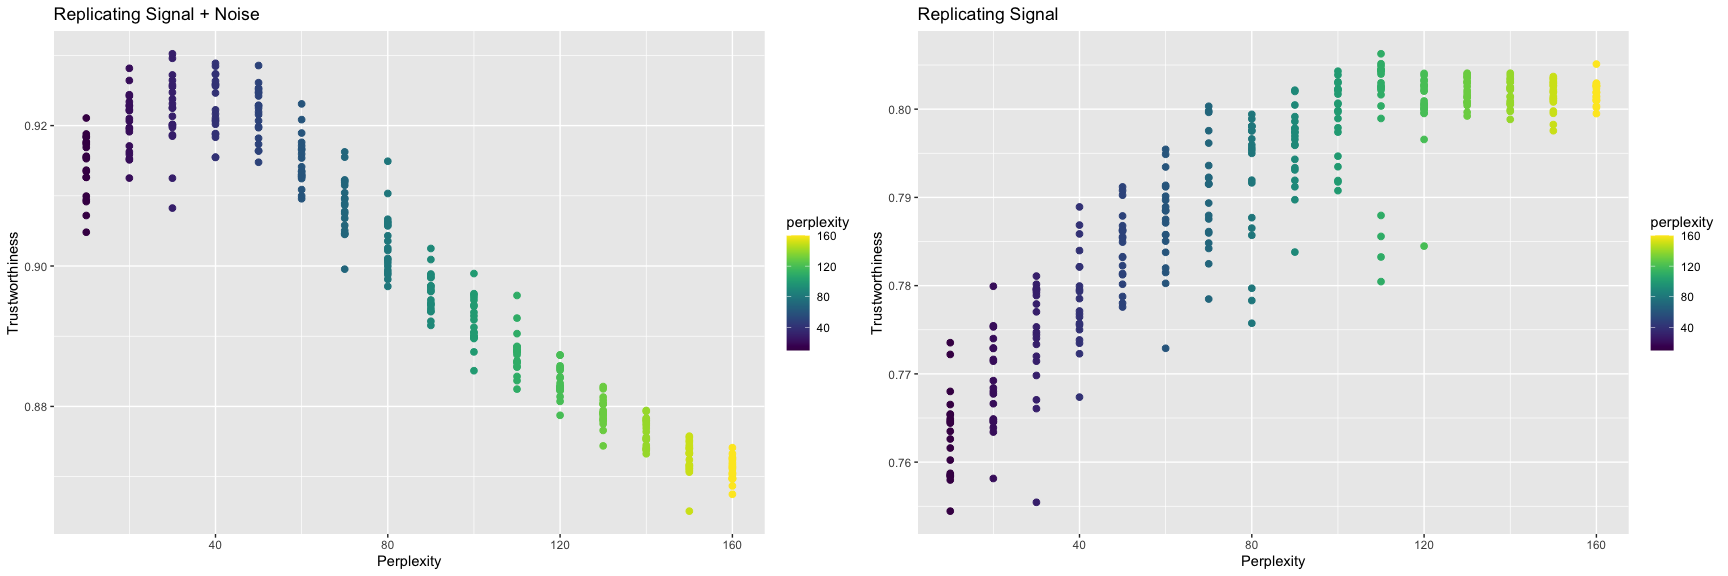
\includegraphics[scale=0.28]{trust plot (trefoil)}
\caption{Trefoil Plots}
\end{figure*}

\begin{figure*}[t]
\centering
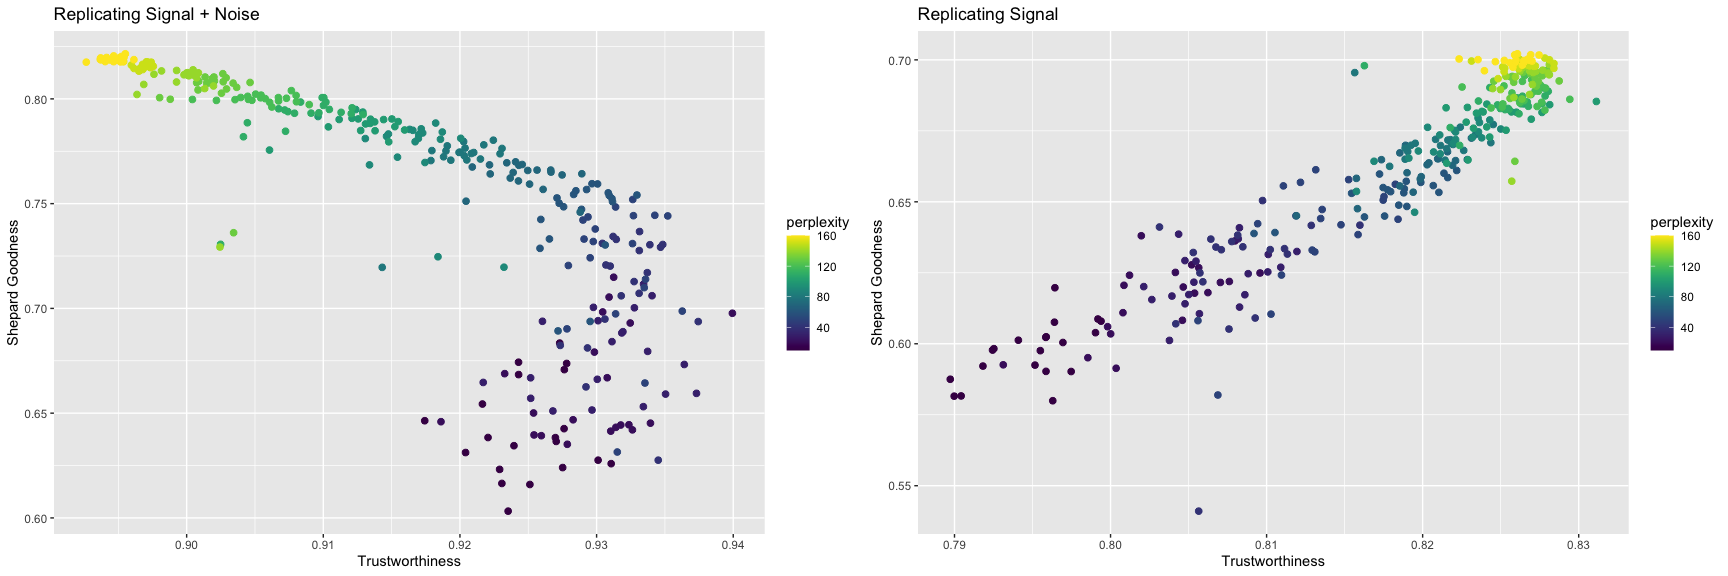
\includegraphics[scale=0.28]{mammoth plot}
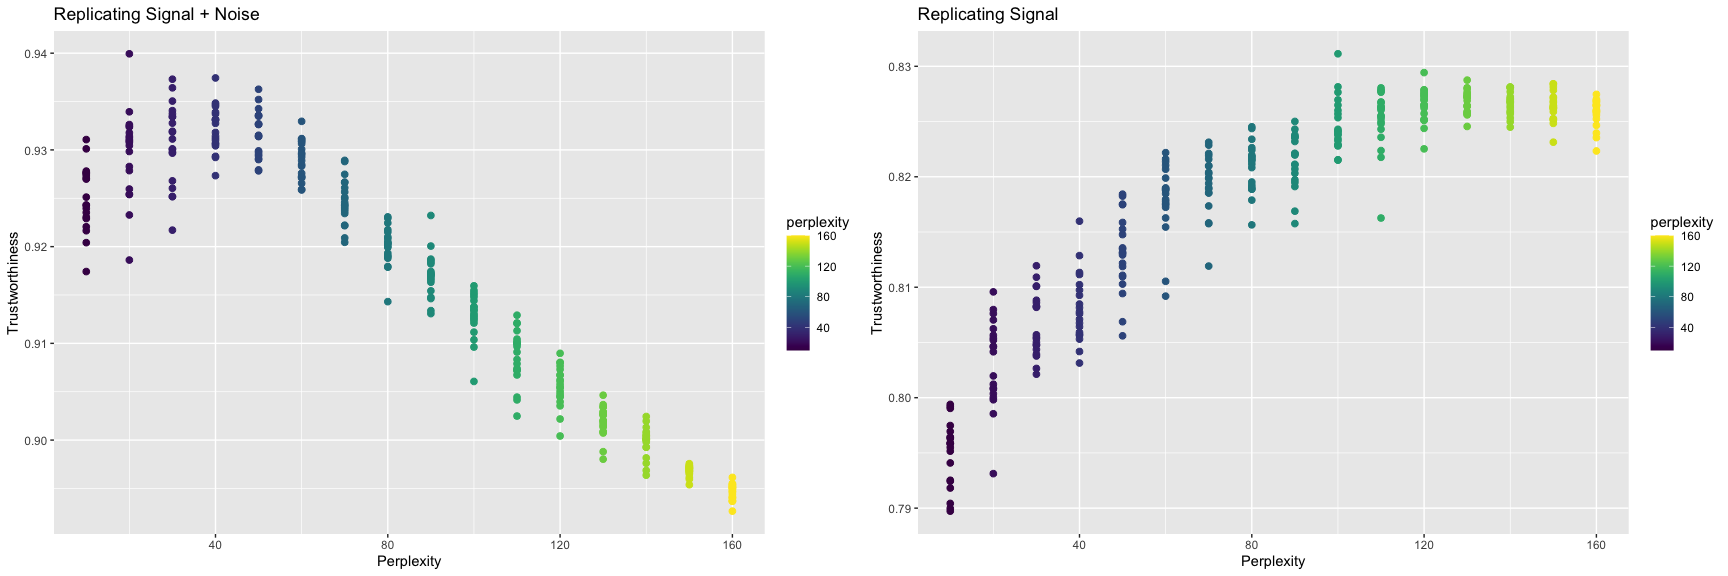
\includegraphics[scale=0.28]{trust plot (mammoth)}
\caption{Mammoth Plots}
\end{figure*}

\begin{figure*}[t]
\centering
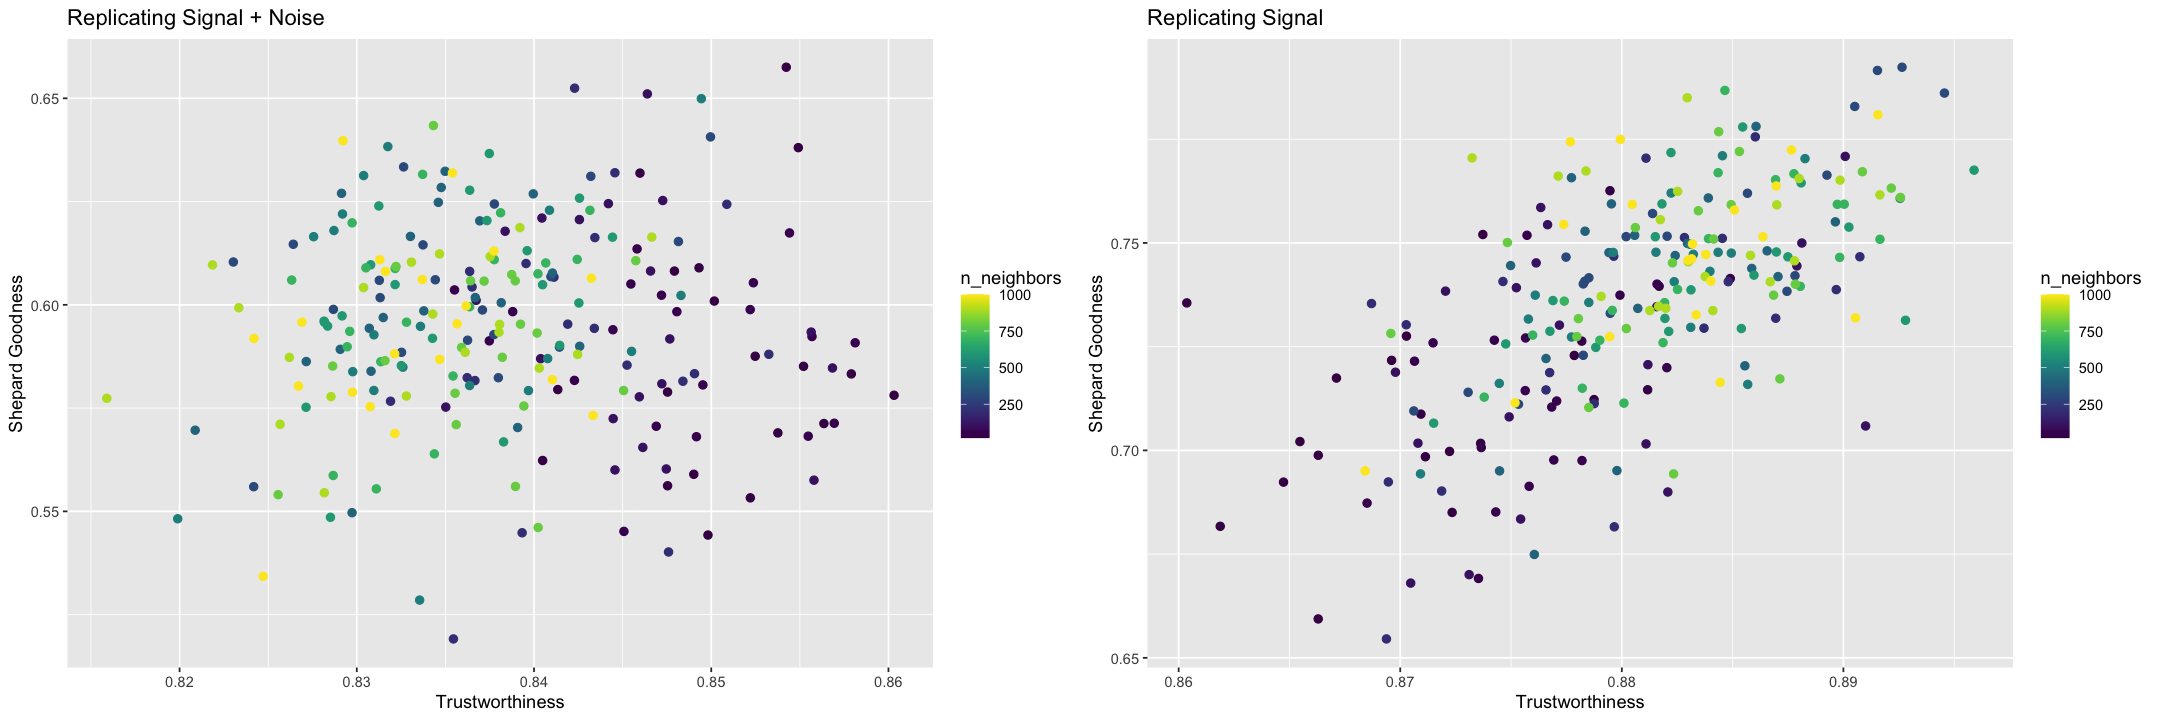
\includegraphics[scale=0.22]{umap plot}
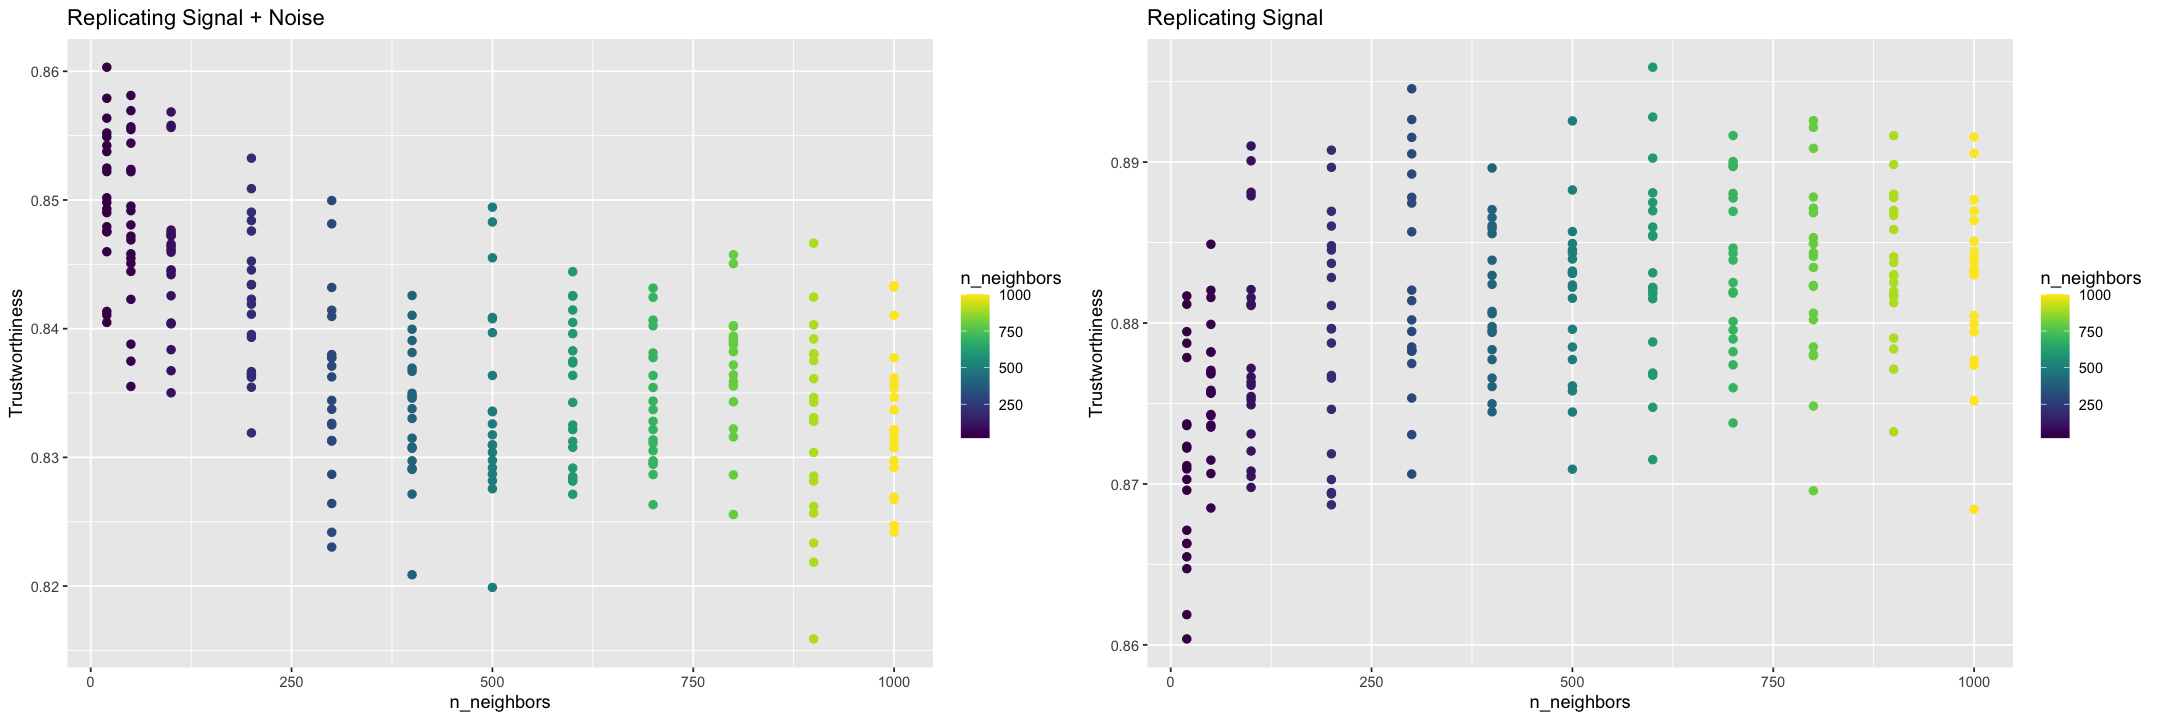
\includegraphics[scale=0.22]{trust plot (umap)}
\caption{UMAP Plots}
\end{figure*}

\end{document}
